\documentclass[11pt,letterpaper]{report}
\usepackage[utf8]{inputenc}
\usepackage[left=1in,right=1in,top=1in,bottom=1in]{geometry}
\usepackage{amsfonts,amsmath}
\usepackage{graphicx,float}
\usepackage{titlesec}
\usepackage{csquotes}
\usepackage{esint}
% -----------------------------------
\usepackage{hyperref}
\hypersetup{%
  colorlinks=true,
  linkcolor=blue,
  citecolor=blue,
  urlcolor=blue,
  linkbordercolor={0 0 1}
}
% -----------------------------------
\usepackage[style=authoryear-icomp,backend=biber]{biblatex}
\addbibresource{citation.bib}
% -----------------------------------
\setlength{\parindent}{0.0in}
\setlength{\parskip}{0.1in}
% -----------------------------------
\input{../command.tex}
% -----------------------------------
\renewcommand\thesection{\arabic{chapter}.\arabic{section}}
\renewcommand\thesubsection{(\arabic{section}.\alph{subsection})}
  
\titleformat{\subsection}[runin]
        {\normalfont\bfseries}
        {\thesubsection}% the label and number
        {0.5em}% space between label/number and subsection title
        {}% formatting commands applied just to subsection title
        []% punctuation or other commands following subsection title
% -----------------------------------
\begin{document}
\begin{titlepage}
    \begin{center}
        \vspace*{4cm}
        \Huge
        \textbf{Recitation Materials} \\
        \vspace{0.5cm}
        \LARGE
        {for NYU Undergraduate Partial Differential Equations}\\
        \vspace{3cm}
        By\\
        \vspace{0.5cm}
        \textbf{Ryan Sh\`iji\'e D\`u}\\
        \vspace{0.2cm}
        \normalsize
        {Courant Institute of Mathematical Sciences - New York University}\\
        \vspace{2cm}
        \Large
        \textbf{Spring, 2023}
        
    \end{center}
\end{titlepage}

\setcounter{tocdepth}{1}
\tableofcontents

\setcounter{chapter}{-1}
% -----------------------------------
\chapter{Before the Course Materials}
%\addcontentsline{toc}{chapter}{READ ME}
%\phantomsection
\section{READ ME}
This document is a compilation of the worksheets used in the recitation sessions for \href{https://math.nyu.edu/dynamic/courses/undergrad/math-ua-263/}{NYU Undergraduate Partial Differential Equations} in Spring of 2023. 

The \LaTeX\ files of this document can be found at \url{https://github.com/Empyreal092/UgradPDE_Worksheet}.

% For students in my recitations: the problems marked with *** are not in the weekly version of the worksheets. They are extra problems.

\chapter{Transport Equations}
\section{Domain of dependence}
[From \cite{Olver_14}, Exercise 2.2.12] A sensor situated at position $x=1$ monitors the concentration of a pollutant $u(t,1)$ as a function of $t$ for $t\geq 0$. Assuming that the pollutant is transported with wave speed $c=3$, at what locations $x$ can you determine the initial concentration $u(0,x)$? 

Remark: this is a first example of an inverse problem. To explain a sub-class of inverse problems: ``forward'' problem is the evolution of the PDE from the initial condition, and inverse problem tries to infer information about the initial condition from observations of the solution at a later time (and a specific location). Things get significantly more difficult when diffusion, modeled by the heat equation, is in the dynamics. Inverse problem is a big field with active research. We will come back to explore more of it later on.

\section{Initial and boundary conditions}
[From \cite{Olver_14}, Exercise 2.2.14] Let $c>0$. Consider the uniform transport equation
\begin{align}
    u_t+cu_x = 0
\end{align}
restricted to the quarter-place $Q = \{x>0, t>0\}$ and subject to initial conditions
\begin{align}
    u(0,x) = f(x) \qdt{for} x\geq 0
\end{align}
along with the boundary condition
\begin{align}
    u(t,0) = g(t) \qdt{for} t\geq 0.
\end{align}

\subsection{}
For which initial and boundary conditions does a classical solution to this initial-boundary value problem exists? Write down a formula for the solution.

\subsection{}
On which regions are the effects of the initial conditions felt? What about the boundary conditions? Is there any interaction between the two?

\section{Blow-up of solution}
[From \cite{ShearerLevy_15}, Exercise 3.8] 

\subsection{}
Use the method of characteristics to solve the initial value problem: 
\begin{align}
    u_t+tu_x = u^2,\quad -\infty<x<\infty,\; 0<t<1
\end{align}
with initial condition 
\begin{align}
    u(x,0) = \frac{1}{1+x^2}.
\end{align}

\subsection{}
Show that the solution blows up as $t\to 1^-$:
\begin{align}
    \lim_{t\to 1^-} \max_x u(x,t) = \infty.
\end{align}

Remark: for a similar problem, see \cite[Exercise 2.2.11]{Olver_14}.

\chapter{Wave Equations}
\section{Symmetries of the wave equation}
[From \cite{ShearerLevy_15}, Exercise 4.3] Show that if $u(x,t)\in C^3$ is a solution of the wave equation
\begin{align}
    u_{tt} = c^2u_{xx},
\end{align}
then so are the following functions:

\subsection{}
For any $y\in\mathbb{R}$, the function $u(x-y,t)$

\subsection{}
Both $u_x$ and $u_t$.

\subsection{}
For any $a\in\mathbb{R}$, the function $u(ax,at)$. 

\section{Domain of dependence}
[From \cite{ShearerLevy_15}, Exercise 4.6] Suppose $u$ satisfies the wave equation with $c=1$ for $x>0$. We want to find a solution of the PDE for $x>0, t>0$, that satisfy the initial conditions
\begin{align}
    & u(x,0) = \phi(x)\\
    & u_t(x,0) = \psi(x),
\end{align}
and the boundary condition
\begin{align}
    u_x(0,t) = 0.
\end{align}

\subsection{}
Solve for $u(x,t)$

\subsection{}
Assume $\supp\phi = \supp\psi=[1,2]$, where can you guarantee that $u=0$ for $x>0, t>0$. 

\section{Fourier series and the expansions of $\pi$}
\subsection{}
Show the Fourier series of periodic extension of $x$ on the interval $(-\pi,\pi)$ is
\begin{align}
    x = \sum_{n=1}^\infty \frac{2(-1)^{n+1}}{n}\sin(nx).
\end{align}

\subsection{}
Show this expansion of $\pi$:
\begin{align}
    \frac{\pi}{4} = 1-\frac{1}{3}+\frac{1}{5}-\frac{1}{7}+\dots
\end{align}

\subsection{}
Show the solution to the Basel problem is
\begin{align}
    1+\frac{1}{4}+\frac{1}{9}+\frac{1}{16} + \dots = \frac{\pi^2}{6}.
\end{align}

\section{Challenging wave equation problem}
[From Spring 2019 of Applied Differential Equations qualifying exam at UCLA, Problem 1\footnote{\url{https://ww3.math.ucla.edu/wp-content/uploads/2021/09/ade-19S.pdf}}]  Let $u(x,t)$ solve the initial value problem
\begin{align}
    \begin{cases}
        u_{tt}+u_{xt}-2u_{xx} = 0,\quad x\in\mathbb{R}, t>0,\\
        u(x,0) = g(x),\\
        u_t(x,0) = h(x).
    \end{cases}
\end{align}

\subsection{}
Derive a formula for $u$ in terms of $g$ and $h$, when $g$ and $h$ are $C^2$. 

Hint: Consider how to simplify the equation into something more obviously like the wave equation
by making a change of coordinate system: $(x,t)\to (\zeta,t)$ where $\zeta = x-vt$ for $v$ appropriately determined. 

\subsection{}
Next consider the boundary value problem 
\begin{align}
    \begin{cases}
        u_{tt}+u_{xt}-2u_{xx} = 0,\quad x\in[0,1], t>0,\\
        u(0,t) = u(1,t) = 0.
    \end{cases}
\end{align}
Show that a smooth solution $u$ to above problem must be zero if $u(x,0)=u_t(x,0)=0$. 

Hint: use an energy argument. Try the energy for the wave equation. 

\section{Stokes' rule***}
[From \cite{Evans_10}, Exercise 2.18]

\section{Equipartition of energy}
[From \cite{Evans_10}, Exercise 2.24] Let $u$ solve the initial-value problem for the wave equation in one dimension:
\begin{align}
    u_{tt}-u_{xx} = 0 &\qdt{in} \mathbb{R}\times(0,\infty)\\
    u=0, u_t=0 &\qdt{on} \mathbb{R}\times\{t=0\}.
\end{align}
Suppose $g,h$ have compact support. We define the kinetic energy
\begin{align}
    k(t):= \frac{1}{2}\int_{-\infty}^\infty u_t^2(x,t)\;\de x
\end{align}
and the potential energy
\begin{align}
    p(t):= \frac{1}{2}\int_{-\infty}^\infty u_x^2(x,t)\;\de x.
\end{align}
We know that the total energy $k(t)+p(t)$ is constant in $t$. Show that $k(t)=p(t)$ for all large enough times $t$. 

\chapter{Conservation Laws}
\section{First time of shock}
[See \cite{ShearerLevy_15}, \S3.4.1] This is an alternative way to derive the first time of shock for Burgers' equation. We have the Burgers' equation:
\begin{align}
    & u_t + uu_x = 0\label{eq:burgers}\\
    & u(x,0) = g(x).\nonumber
\end{align}

\subsection{}
Take the $x$-derivative of the Burgers' equation and derive an equation for the evolution of $u_x$. We name $v:= u_x$.

\subsection{}
Transform the above PDE into an ODE with a change of variable. Hint: try the Galilean transformation again.

\subsection{}
Solve this ODE and recover the first time of shock result you learned in lecture.

\section{Traveling backwards in traffic law}
We have the Lighthill-Whitham-Richards model for traffic flow
\begin{align}
    \rho_t + F(\rho)_x = 0.
\end{align}
In particular we use the Greenshields model for the flux:
\begin{align}
    F(\rho) = \rho(1-\rho).
\end{align}

\subsection{}
What is the speed of characteristics for the Greenshields model?

\subsection{}
Notice that when the traffic density is large ($\rho>1/2$), the characteristics actually travel backwards (against the direction of flow of cars). Can you explain the backward movement of characteristics physically?

\section{Integral solution to 1D conservation law}
Note: this is above and beyond what you need for this undergraduate level class. We would talk about it only if we have time. But learning the rigorous theory is useful if you need to extend what we learned in this class to a more general context. Test functions will show up later in class. Lastly, thinking about this is a fun intellectual exercise. :)

[See \cite{Evans_10}, \S3.4.1] At a shock, classic notion of solution to a PDE breaks down since we cannot take derivatives of the solution. We must devise some way to interpret a less regular function $u$ as somehow ``solving'' the PDE. The idea of an integral (weak) solution is to transfer the derivatives to a test function $v$ via integration by parts. 

More precisely, assume
\begin{align}
    v: \mathbb{R}\times[0,\infty)\to\mathbb{R} \text{ is smooth ($C^\infty$), with compact support}.\label{eq:test_func}
\end{align}
We say that $u\in L^\infty(\mathbb{R}\times(0,\infty))$ is an integral solution of \eqref{eq:cons_Fu}, if
\begin{align}
    \int^\infty_0\int^\infty_{-\infty} uv_t+F(u)v_x\;\de x\de t+\int^\infty_{-\infty} gv\;\de x|_{t=0} = 0
\end{align}
for all test function $v$ satisfying \eqref{eq:test_func}.

Note: For this to work such $v$ needs to exist. One example of such $v$ is the ``bump function''. Their existence might be surprising for a first-timer, but they are essential tools in analysis of PDE so get used to them.

\subsection{}
Assume $u$ is smooth, use integration by part to show that the above condition for the integral solution is equivalent to the requirement for $u$ to be a classic solution.

Note: here we use a theorem that states: for a continuous function $f$, if $f(x_0)>0$ for some $x_0$, there exists a small ball around $x_0$ such that for all $y\in B(x_0,\epsilon)$, $f(y)>0$. Review your analysis notes, or look this up.

\subsection{}
Now assume that $u$ has a jump. Perform integration by parts again to obtain the Rankine-Hugoniot condition.

To do this, assume $v$ is zero at $t=0$ to make the initial condition term zero. More importantly, the boundary terms from integration by parts are not zero at the jump. They will give you the speed of the shock.

\subsection{}
That was a lot of work. Is this enough? Unfortunately no. The integral solutions are not unique, especially for rarefaction wave. We also need the entropy condition. You will learn this next week.

\section{Burgers' with shock and expansion fan}
Solve the Burgers' equation on the infinite domain with the initial condition:
\begin{align}
    u(x,0) = \begin{cases}
        1 & \text{for\;} 0\leq x\leq 1,\\
        0 & \text{otherwise}.
    \end{cases}
\end{align}

\subsection{}
At $t=0$, what happens at $x=0$? What happens at $x=1$?

\subsection{}
Draw the solution at $t=2$. 

\subsection{}
Continue for solution past $t=2$. Draw the shock curve and some sample characteristic lines in an $x-t$ plot as time progresses. 

\section{Periodic Burgers'}
Solve the Burgers' equation on the periodic $x\in[0,1]$ with the initial condition
\begin{align}
    u(x,0) = \begin{cases}
        1 & \text{for\;} x\in[0,1/2),\\
        0 & \text{for\;} x\in[1/2,1).
    \end{cases}
\end{align}

What happens at time $t=1$? Continue your solution past time $t=1$ and draw the shock curve and some sample characteristic lines in an $x-t$ plot at time progress. 

\section{Green light on a two way street}
[From Esteban Tabak's PDE note\footnote{See the end of note \url{https://math.nyu.edu/~tabak/PDEs/Traffic_flow.pdf}}] I will quote Esteban Tabak for his wonderful description of this traffic phenomenon
\begin{displayquote}
    You are in a long traffic queue in a two-way street--say Park Avenue--waiting for the green light. When the light finally turns green, the first car in the queue moves, then the second, and so on: a wave propagates backward through the queue, telling the cars when to start. On the other hand, you see on your left the first cars moving the opposite way, as they start with the green light at the intersection and soon reach your point in the queue. My observation is--please confirm this with your own experience!--that the time at which the first car going the other way reaches your position in the queue agrees almost exactly with your starting time. 
\end{displayquote}
We will give an explanation of this phenomenon using the Greenshields model for the traffic flux:
\begin{align}
    F(\rho) = \rho(1-\rho).
\end{align}

\subsection{}
What happens in the Greenshields model when the traffic light turns green?

\subsection{}
Calculate the speed of the two ends of the expansion fan.

\section{Red light, green light}
[From \cite{ShearerLevy_15}, \S13.2.1] A line of traffic with uniform density $\overline{\rho}<1/2$ approaches a traffic light located at $x=0$. We start the solution at $t=0$ with the initial condition
\begin{align}
    u(x,0) = \begin{cases}
        \overline{\rho} & \text{for\;} x\leq 0,\\
        0 & \text{for\;} x>0.
    \end{cases}
\end{align}

The traffic light stays red till time $t_1$ and turns green. 

\subsection{}
Solve the traffic problem during $t\in[0,t_1]$. What is the direction of the shock? Does this make sense intuitively?

\subsection{}
Calculate the first time $t>0$ when there is no maximum density $\rho=1$ in the domain. Name this time $t_2$.

\subsection{}
Solve the traffic problem past time $t_2$ by drawing the shock curve and some sample characteristic lines. Will the shock pass $x=0$ again? 

$t_3-t_1$ is the shortest a well-designed green light should last. After that the traffic behind the traffic light is restored to the incoming density $\overline{\rho}$ and the cycle continues.

\section{Deriving expansion fan solutions from scaling symmetry}
We solve the Riemann problem for a conservation law with strictly convex flux $F(u)$:
\begin{align}
    & u_t+F(u)_x = 0\\
    & u(x,0) = \begin{cases}
        u_L &\text{for }x<0\\
        u_R &\text{for }x\geq 0
    \end{cases}.
\end{align}

\subsection{}
What is the relation between $u_L$ and $u_R$ that admits an expansion fan solution, instead of a shock solution that satisfy the Lax stability criterion. 

\subsection{}
Show that the change of variable $\tau=at$, $y=ax$ does not change the Riemann problem. 

\subsection{}
This scaling symmetry inspires us to look for solution of the form $u(x,t) = \phi(\zeta)$ where $\zeta = x/t$. Plug this ansatz into the Riemann problem to find out what $\phi$ should be.

\subsection{}
Put all the pieces together and obtain the expansion fan solution
\begin{align}
    u(x,t) = \begin{cases}
        u_L &\text{if } x \leq F'(u_L) t, \\
        (F')^{-1}(x/t) &\text{if } F'(u_L) t \leq x \leq F'(u_R) t, \\
        u_R &\text{if } F'(u_R) t \leq x.
    \end{cases}
\end{align}

\chapter{Heat Equation}
\section{Heat flux and the Robin boundary condition}
\subsection{}
Write the heat equation as a conservation law. What is the heat flux function? 

Relating the flux to its gradient is called the Fourier's law or the Fick's law.

\subsection{}
Imagine we have a metal rod where one end of it is submerged in cold water. The water has temperature $T_L$ and is moving. The heat flux due to convection is
\begin{align}
    q = h(T-T_L)
\end{align}
where $h$ is called the convection coefficient.

This heat flux must be equal to the heat flux at the end of rod which follows the Fourier's law. From this obtain that $\theta = T-T_L$ must satisfy the homogeneous robin boundary condition.

% \section{Application of the fundamental solution to solve Dirichlet problems}
% \subsection{}
% Error function

% \subsection{}
% Combine them

% \subsection{}
% [From \cite{Olver_14}, Problem 8.1.1]

\section{Alternative statements of the method of images}
[From \cite{ShearerLevy_15}, Problem 5.3] We have $\Phi$ the fundamental solution of the heat equation.

\subsection{}
Let $g:[0,\infty)\to\mathbb{R}$ be a bounded integrable function. Prove directly that
\begin{align}
    u(x,t)=\int_0^\infty (\Phi(x-y,t)-\Phi(x+y,t))g(y)\;\de y
\end{align}
is an odd function of $x\in\mathbb{R}$ for each $t>0$.

\subsection{}
Let $h:\mathbb{R}\to\mathbb{R}$ be an odd bounded integrable function. Prove that
\begin{align}
    u(x,t)=\int^\infty_{-\infty} \Phi(x-y,t)h(y)\;\de y
\end{align}
is an odd function of $x\in\mathbb{R}$ for each $t > 0$. That is, the symmetry in the initial data is carried through to the same symmetry in the solution.

\section{Maximum and variance of the fundamental solution}
[Adapted from \cite{Olver_14}, Problem 8.1.6]

\subsection{}
What is the maximum value of the fundamental solution at time $t$?

\subsection{}
Calculate the ``variance'' of the fundamental solution:
\begin{align}
    \var(u(t)) = \int_\mathbb{R} x^2 u(t,x)\;\de x.
\end{align}
One could do this directly. Alternatively, calculate how the variance change in time:
\begin{align}
    \frac{\de}{\de t}\var(u(t)) = \frac{\de}{\de t}\int_\mathbb{R} x^2 u(t,x)\;\de x.
\end{align}

\subsection{}
Can you justify the claim that its width is proportional to $\sqrt{t}$?

\section{Advection-diffusion equation}
[From \cite{ShearerLevy_15}, Problem 5.10] Devise a change of variable corresponding to a moving frame of reference to solve the initial value problem for the advection-diffusion equation with constant speed $c$
\begin{align}
    &u_t+cu_x = ku_{xx},\quad -\infty<x<\infty, t>0,\\
    &u(x,0) = g(x),\quad -\infty<x<\infty
\end{align}

\section{Heat equation with damping}
[From \cite{ShearerLevy_15}, Problem 5.9] Consider the initial value problem
\begin{align}
    &u_t+du = ku_{xx},\quad -\infty<x<\infty, t>0,\\
    &u(x,0) = g(x),\quad -\infty<x<\infty
\end{align}
with constant $d$, and given integrable function $g$.

\subsection{}
Use the change of variable $u(x, t) = e^{-dt}v(x,t)$ to find $u$ using the
fundamental solution.

\subsection{}
What is the effect of the constant $d$?

\subsection{}
Suppose $d = d(t)$ is a given continuous function. What would be a suitable
change of variable to solve the problem?

\section{Properties of convolution}\label{sec:p1}
\subsection{}
Convolution of two Gaussians is still a Gaussian: take $f(x) = e^{-ax^2}$ and $g(x) = e^{-bx^2}$, calculate explicitly $f*g$ and show that it is still a Gaussian.

Hint: complete the square.

Remark: More generally, suppose $f$ is the probability density function (PDF) of Gaussian random variable with mean $\mu_1$ and variance $\sigma_1^2$, and $g$ with mean $\mu_2$ and variance $\sigma_2^2$, their convolution $f*g$ is the PDF of Gaussian random variable with mean $(\mu_1+\mu_2)$ and variance $(\sigma_1^2+\sigma_2^2)$. But calculating this explicitly is cumbersome. It is easier to show this using Fourier transform (FT), where the FT of Gaussian is still Gaussian, and the FT of convolution is the product of the two FTs (the convolution theorem). That is:
\begin{align}
    \mathcal{F}(f*g) = \mathcal{F}(f)\cdot \mathcal{F}(g)
\end{align}
where $\mcal{F}$ deotes the Fourier transform.

\subsection{}
Convolution is associative: show that
\begin{align}
    (f*g)*h = f*(g*h).
\end{align}

\section{Continuous space, discrete time random walk}
Instead of taking a step on a grid, we imagine a random walk on continuous $\mathbb{R}$. Suppose the walker starts off at $0$, at the next timestep of size $\Delta t$, the walker will be at location $\Delta x$ with probability
\begin{align}
    p(\Delta x) = \frac{1}{ \sqrt{2\pi d\Delta t} } e^{-\frac{1}{2}\frac{\Delta x^2}{d\Delta t}}.
\end{align}
That is, the probability that the walker will move $\Delta x$ is a centered Gaussian random variable with variance $d\Delta t$. This is a continuous space version of discrete random walk.

\subsection{}
Assume at initial time the probability that the walker is located at $x_0$ follows PDF $f(x_0)$, what is the probability that it will be at $y$ after a $\Delta t$ step?

Remark: $y$ is a random variable that is the sum of $x_0$ and $\Delta x$, which themselves are random variables. We just shown that the PDF of $y$ is the convolution of the PDF of $x_0$ and the PDE of $\Delta x$. This is true for the sum of any two independent random variables.

\subsection{}
Take another step of $\Delta t'$, use the facts in Problem \ref{sec:p1} to write the probability of the walker to be at $y$ after the combined $\Delta t+\Delta t'$ step without explicit calculation.

\subsection{}
Relate the above formula to the heat kernel and thus show that in the limit of continuous time, the PDF evolves following the heat equation.

\subsection{}
This example is special because the PDF of the step is Gaussian. How about more general PDFs? How about the discrete random walk? Under mild conditions (the step has zero mean and finite variance), the sum of many independent walks converges to a Gaussian. This is due to the central limit theorem(CLT):
\begin{displayquote}
    Suppose $\{X_{1},\ldots ,X_{n},\ldots \}$ is a sequence of independent and identically distributed (i.i.d.) random variables with $\mathbb {E} [X_{i}]=\mu$ and $\var[X_{i}]=\sigma ^{2}<\infty$. Then as $n$ approaches infinity, the sum of $(1/\sqrt {n}) (X_n-\mu)$ converges in distribution to a normal $\mathcal {N}(0,\sigma ^{2})$:
    \begin{align}
        \frac{1}{\sqrt{n}}\sum_{i=1}^n (X_i-\mu) \xrightarrow{d} \mathcal {N}(0,\sigma ^{2}).
    \end{align}
\end{displayquote}
The theorem shows the importance of Gaussian random variable as it naturally arises from the sum of i.i.d. random variables. This is why reason the Gaussian is ubiquitous in nature (e.g.: the evolution of heat). 

Now use this theorem to relate (informally) the discrete random walk to the heat equation.

Remark: this is a different approach to show the (space and time) continuous limit of discrete random walk follows the heat equation. You could check the answer of your solution to the HW problems using this line of thinking.

\section{Stability requirement of finite difference schemes}
In the HW you will show that an explicit finite difference scheme for the heat equation have the requirement for the time step size $\Delta t$ to be proportional to $\Delta x^2$. This means we need \emph{very} small time steps if the spatial resolution is fine ($\Delta x$ is small). However, this is an inescapable requirement for explicit method for the heat equation. We will understand this using the domain of dependence of the heat equation.

\subsection{}
Convince yourself that the domain of dependence of the heat equation is the whole domain.

\subsection{}
Now we calculate the numerical domain of dependence. Here we define the numerical domain of dependence at time $T$ and grid point $X$ to be the spatial grid points at time $0$ that influence the result at $(T,X)$.

Assume that $\Delta t$ is proportional to $\Delta x$, how does the numerical domain of dependence change as $\Delta x\to 0$? How about if $\Delta t$ is proportional to $\Delta x^2$?

\subsection{}
The necessary condition for the stability of a finite difference scheme is that its numerical domain of dependence should include the actual domain of dependence of the PDE as $\Delta x\to 0$. We can understand this as a restatement of interpolation is stable while extrapolation is not. Therefore an explicit scheme for the heat equation cannot have $\Delta t$ proportional to $\Delta x$. 

Remark: One way out of this is to use an implicit timestepping scheme.

\chapter{Dispersive Waves}
\section{Alternative formula for Fourier transform}
In the HW you have one definition of the Fourier transform and its associated inversion formula:
\begin{align}
    &\hat f(\xi) = \int f(x)e^{-i\xi x} \;\de x,\\
    &f(x) = \int \hat f(\xi)e^{+i\xi x} \;\de \xi \cdot\frac{1}{2\pi}.
\end{align}
An alternative formula that absorbs the $2\pi$ factor into the Fourier kernal is:
\begin{align}
    &\hat f(\xi ) = \int f(x)e^{-2\pi i\xi x} \;\de x,\\
    &f(x) = \int \hat f(\xi)e^{+2\pi i \xi x} \;\de \xi \label{eq:Four_inv}.
\end{align}
Show that they are equivalent. I would use the second version in this note.

\section{Poisson summation formula}
[From \cite{SteinShakarchi_03}, \S5.3] Given a Schwartz function $f$ on the real line, we can construct a new periodic (with period 1) function on the circle by the recipe
\begin{align}
    F_1(x) = \sum_{n=-\infty}^\infty f(x+n).
\end{align}
Another way is by Fourier analysis. Start with \eqref{eq:Four_inv} and consider its discrete analogue, where the integral is replaced by a sum:
\begin{align}
    F_2(x) = \sum_{n=-\infty}^\infty \hat f(n)e^{2\pi inx}.
\end{align}
A technical note, both of these sum are convergent absolutely and uniformly (for any compact interval) because of the assumption that $f$ is in the Schwartz space. Therefore, they are continuous. 

\subsection{}
Show that the two approaches are the same. That is, show the Poisson summation formula
\begin{align}
    \sum_{n=-\infty}^\infty f(x+n) = \sum_{n=-\infty}^\infty \hat f(n)e^{2\pi inx}.
\end{align}
In particular we have the corollary
\begin{align}
    \sum_{n=-\infty}^\infty f(n) = \sum_{n=-\infty}^\infty \hat f(n).
\end{align}

Hint: Show both sides (which are periodic) have the same Fourier series. Then the function is the same because Fourier series are unique for continuous function.

\subsection{Heat kernels} We have the heat kernel for the heat equation (with coefficient 1) on $\mathbb{R}$:
\begin{align}
    \mcal{H}_t(x) = \frac{1}{(4\pi t)^{1/2}}e^{-x^2/4t}
\end{align}
which has the Fourier transform
\begin{align}
    \hat{\mcal{H}}_t(\xi) = e^{-4\pi^2 \xi^2 t}.
\end{align}
You also derived the heat kernel on a periodic interval of length 1:
\begin{align}
    H_t(x) = \sum_{n=-\infty}^\infty e^{-4\pi^2 n^2 t}e^{2\pi inx}.
\end{align}
Using the Poisson summation formula, show that the periodic heat kernel is the periodization of the
heat kernel on the real line:
\begin{align}
    H_t(x) = \sum_{n=-\infty}^\infty \mcal{H}_t(x+n).
\end{align}

\section{Nyquist–Shannon sampling theorem}
[From Problem 7.6 of \cite{ShearerLevy_15}] This is one of the fundamental theorem in signal processing. Consider the Fourier transform of a band-limited Schwartz function $f(x)$, in which $\hat f(\xi) = 0$ for $|\xi|>1/2$. 

\subsection{}
Show
\begin{align}
    \hat{f}(\xi)=\sum_{-\infty}^\infty f(n)e^{-2\pi in \xi}
\end{align}
for $\xi\in [-1/2, 1/2]$. 

\subsection{}
Hence deduce that $f(x)$ only depends on the sequence $\{f(n)\}$ of sampled values of $f$:
\begin{align}
    f(x) = \sum_{n=\infty}^\infty f(n) \text{sinc}(x-n)\label{eq:WhSh_form}
\end{align}
where $\text{sinc}$ is the normalized sinc function where
\begin{align}
    \text{sinc}(x) = \frac{\sin(x)}{x}.
\end{align}

Remark: \eqref{eq:WhSh_form} is called the Whittaker–Shannon interpolation formula.

\subsection{}
[From Problem 5.20(c) of \cite{SteinShakarchi_03}] Prove that
\begin{align}
    \int_\infty ^\infty |f(x)|^2\;\de x = \sum_\infty ^\infty |f(n)|^2.
\end{align}

\subsection{}
We now add dimension into the statement to make it more applicable to the real world. We use time here but space is just as valid. Shannon's version of the theorem states \parencite{Shannon_49}:
\begin{displayquote}
    If a function $f(t)$ contains no frequencies higher than $W$ cps, it is completely determined by giving its ordinates at a series of points spaced $1/2W$ seconds apart.
\end{displayquote}
The threshold $2W$ is called the Nyquist rate and is an attribute of the continuous-time input $x(t)$ to be sampled. The sample rate must exceed the Nyquist rate for the samples to suffice to represent $x(t)$. Thinking from the sampling equipment's perspective: The threshold $f_{s}/2$ is called the Nyquist frequency and is an attribute of the sampling equipment. All meaningful frequency components of the properly sampled $x(t)$ exist below the Nyquist frequency. 

What happens if the signal has higher frequencies than our sampling allows? What if the signal is not band limited at all? You have seen the consequences when you try to take a picture of the computer screen. You would see aliasing.
\begin{figure}[H]
    \centering
    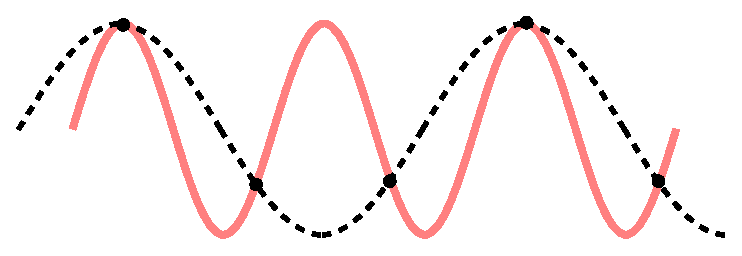
\includegraphics[width = 0.5\textwidth]{../Session_8/figs/alias}
\end{figure}

\section{The Heisenberg uncertainty principle}
[From \S5.4 of \cite{SteinShakarchi_03}] Suppose $\psi$ is a Schwartz function which satisfies the normalizing condition
\begin{align}
    \int_\infty^\infty |\psi(x)|^2 \;\de x = 1.\label{eq:normaliz}
\end{align}

\subsection{}
Show that
\begin{align}
    \left( \int_\infty^\infty x^2|\psi(x)|^2 \;\de x \right)\left( \int_\infty^\infty \xi^2|\hat\psi(\xi)|^2 \;\de \xi \right) \geq \frac{1}{16\pi^2}.
\end{align}
In fact, we have
\begin{align}
    \left( \int_\infty^\infty (x-x_0)^2|\psi(x)|^2 \;\de x \right)\left( \int_\infty^\infty (\xi-\xi_0)^2|\hat\psi(\xi)|^2 \;\de \xi \right) \geq \frac{1}{16\pi^2}.
\end{align}

Hint: start from \eqref{eq:normaliz}, integrate by parts. Remember to use the Cauchy-Schwarz inequality and the Plancherel formula (Parseval identity). 

Remark: You might recognize $|\psi(x)|^2$ as a probability distribution and we have the variance of $|\psi(x)|^2$ and $|\hat\psi(\xi)|^2$. The interpretation of this result in quantum mechanics is:
\begin{align}
    \text{(uncertainty of position)}\times\text{(uncertainty of momentum)} \geq \frac{\hbar}{16\pi^2}
\end{align}
where $\hbar$ is the Planck's constant. If you know a bit of quantum mechanics or is interested, I encourage you to work through Problem 5.23 of \cite{SteinShakarchi_03}. 

\subsection{}
[From Problem 5.21 of \cite{SteinShakarchi_03}] Another statement of the uncertainty principle is: suppose that $f$ is continuous on $\mathbb{R}$. Show that $f$ and $\hat f$ cannot both be compactly supported unless $f = 0$. 

Hint: Assume $f$ is supported in $[0, 1/2]$. Expand $f$ in a Fourier series in the
interval $[0, 1]$, and note that as a result, $f$ is a trigonometric polynomial.

\section{Alternative formula for Fourier transform}
In the HW you have one definition of the Fourier transform and its associated inversion formula:
\begin{align}
    &\hat f(\xi) = \int f(x)e^{-i\xi x} \;\de x,\\
    &f(x) = \int \hat f(\xi)e^{+i\xi x} \;\de \xi \cdot\frac{1}{2\pi}.
\end{align}
An alternative formula that absorbs the $2\pi$ factor into the Fourier kernal is:
\begin{align}
    &\hat f(\xi ) = \int f(x)e^{-2\pi i\xi x} \;\de x,\\
    &f(x) = \int \hat f(\xi)e^{+2\pi i \xi x} \;\de \xi \label{eq:Four_inv}.
\end{align}
Show that the second version is also valid. I would use the second version in this note.

\section{Some example dispersion relations}
\subsection{}
The Korteweg–De Vries equation is a nonlinear, dispersive PDE that models waves on shallow water surfaces
\begin{align}
    u_t+u_{xxx}-6uu_x = 0.
\end{align}
It is clear that zero is a solution. Linearize the equation around the zero solution. That is, assume the amplitude of the solution is small. We get
\begin{align}
    w_t+w_{xxx} = 0.
\end{align}
What is the dispersion relation? What is the phase velocity and group velocity?

\subsection{}
Kuramoto-Sivashinsky equation or the flame equation model a flame front. 
\begin{align}
    u_t+u_{xx}+u_{xxxx}+\frac{1}{2}u_x^2 = 0.
\end{align}
It is known for its chaotic behavior. Again linearize around the zero solution to get the linear PDE
\begin{align}
    w_t+w_{xxxx}+w_{xx} = 0.
\end{align}
Calculate the same three quantities.

\subsection{}
We study the sine-Gordon equation
\begin{align}
    u_{tt} = c^2u_{xx}-\sin(u).
\end{align}
Linearize around the zero solution. Calculate the same three quantities.

\section{Numerical diffusion and dispersion}
[From \S10.9 of \cite{LeVeque_07}] We will study finite difference scheme for the advection equation
\begin{align}
    u_t+au_x = 0.
\end{align}
We assume $a>0$ and $a=O(1)$. 

\subsection{}
We could use the upwinding scheme
\begin{align}
    U^{n+1}_j = U^n_j-\frac{a\Delta t}{\Delta x}\left( U^n_j-U^n_{j-1} \right).
\end{align}
Show that the upwinding scheme is a consistent approximation of the PDE using Taylor expansion. 

\subsection{}
Take a function $v(x,t)$ that satisfy the upwinding scheme exactly:
\begin{align}
    v(x,t+\Delta t)=v(x,t)-\frac{a\Delta t}{\Delta x}\left[v(x,t)-v(x-\Delta x,t)\right].
\end{align}
Show that up to an $O(\Delta t^2)$ approximation the PDE that $v$ satisfies is
\begin{align}
    v_t+av_x = \frac{1}{2}a\Delta x\left(1-\frac{a\Delta t}{\Delta x}\right)v_{xx}.
\end{align}
This is called the modified equation of the upwinding scheme.

Therefore the numerical error when we use the upwinding scheme is diffusive in nature.

\begin{figure}[H]
    \centering
    \includegraphics[width=0.8\textwidth]{../Session_9/figs/num_dispers}
\end{figure}

\subsection{}
A better approximation to the advection equation gives the Lax-Wendroff scheme:
\begin{align}
    U^{n+1}_j = U^n_j-\frac{a\Delta t}{2\Delta x}\left( U^n_{j+1}-U^n_{j-1} \right)+\frac{a^2 \Delta t^2}{2\Delta x^2}\left(U^n_{j+1}-2U^n_{j}+U^n_{j-1}\right).
\end{align}
A rather long calculation\footnote{see \url{https://guillod.org/teaching/m2-b004/TD2-solution.pdf}} gives the modified equation of the Lax-Wendroff scheme:
\begin{align}
    v_t+av_x +\frac{1}{6}a\Delta x^2\left(1-\left(\frac{a\Delta t}{\Delta x}\right)^2\right)v_{xxx} = 0.
\end{align}
Calculate the dispersion relationship for waves in this PDE. Are the waves dispersive? What is the group velocity? We say that the error for the Lax-Wendroff is dispersive in nature. 

For stability, we require the ratio
\begin{align}
    \frac{a\Delta t}{\Delta x}<1.
\end{align}
Compare the group velocity to the advection velocity. Use this to explain the trailing wavy error in the above figure for Lax-Wendroff. 

\subsection{}
The above plot also show the Leapfrog scheme, which also has dispersive error. Another scheme is the Beam-Warming scheme. We see from the figure below that its error is also dispersive, but the error lead the solution. You could do the same calculation and see that $c_g>a$. 
\begin{figure}[H]
    \centering
    \includegraphics[width=0.6\textwidth]{../Session_9/figs/beamwarming}
\end{figure}


\section{Riemann-Lebesgue Lemma}
The mathematical theorem that is behind the method of stationary phase is the Riemann-Lebesgue Lemma. 
\begin{displayquote}
    Let $f:\mathbb{R}\to\mathbb{R}$ be a (Lebesgue) integrable function. Then we have
    \begin{align}
        \lim_{\xi\to\infty} \int^\infty_{-\infty} f(x)e^{i\xi x}\;\de x = 0
    \end{align}
\end{displayquote}
Intuitively, as $\xi$ increases the oscillations in the integral increase and become much faster than any variation in $f(x)$; successive oscillations thus cancel and the integral becomes very small.

\subsection{}
Show this result assuming $f(x)$ is the indicator function for some compact set. Extend the result to step functions which is piecewise constant. 

\subsection{}
Compact (Lebesgue) integrable function can be approximated arbitrary well by step functions. That is, for all $\epsilon>0$ there is a step function $\varphi$ such that
\begin{align}
    \left| \int_M f \;\de x - \int_M \varphi \;\de x \right| < \epsilon.
\end{align}
Use this fact to show that the Riemann-Lebesgue Lemma holds for compact (Lebesgue) integrable function.

\subsection{}
Finally, show that Riemann-Lebesgue Lemma holds for any (Lebesgue) integrable function. That is, function such that
\begin{align}
    \int_\mathbb{R} |f|\;\de x < \infty.
\end{align}

\section{Conservation laws of KdV}
[From \cite{ShearerLevy_15}, Problem 12.2] Given the KdV equation
\begin{align}
    u_t+uu_x+\gamma u_{xxx} = 0
\end{align}
with the condition that the solution decays sufficiently rapidly as $|x|\to\infty$.

\subsection{}
Show that the momentum and kinetic energy (when $u$ interpreted as a velocity) are conserved:
\begin{align}
    \int_\mathbb{R} u\;\de x; \qquad \int_\mathbb{R} u^2\;\de x.
\end{align}

\subsection{}
Find $\eta$ (depending on $\gamma$) so that the integral
\begin{align}
    \int_\mathbb{R} \frac{1}{2}(u_x^2-\eta u^3)\;\de x
\end{align}
is conversed. 

\chapter{Laplace and Poisson Equations}
\section{Poisson’s equation with Robin boundary conditions}
[From \cite{ShearerLevy_15}, Problem 8.3]
Consider Poisson’s equation on a bounded open set $U \in\mathbb{R}^n$ with Robin boundary conditions
\begin{align}
    &\nabla^2 u = f(\ve x),\quad\ve x\in U,\\
    &\qdt{with} \frac{\pe u}{\pe\ve n}+\alpha u(\ve x) = g(\ve x),\quad\ve x\in\pe U.
\end{align}

\subsection{}
Prove that if $\alpha > 0$, then the energy method can be used to show
uniqueness of solutions $u\in C^2(U)\cap C(\overline{U})$

\subsection{}
For $\alpha = 0$, show that solutions are unique up to a constant.

\subsection{}
Design an example to show that uniqueness can fail if $\alpha < 0$. (Hint: Choose $n = 1$.)

\section{Separation of variables for the Helmholtz equation}
[From \cite{Olver_14}, Problem 4.3.18] Use separation of variables to solve the Helmholtz boundary value problem on the unit square:
\begin{align}
    &\nabla^2 u = k^2u\\
    &\qdt{with} u(x,0)=0, u(x,1)=f(x), u(0, y) = 0, u(1, y) = 0
\end{align}

\section{Energy minimization}
[From Fall 2015 of Applied Differential Equations qualifying exam at UCLA, Problem 7\footnote{\url{https://ww3.math.ucla.edu/wp-content/uploads/2021/09/ade-15F.pdf}}] 
Consider $K$ be the set of functions $u: [0, 2] \to \mathbb{R}$ of the form 
\begin{align}
    u(x) = \begin{cases}
        v(x)\qdt{for} x\in[0,1)\\
        w(x)\qdt{for} x\in(1,2]
    \end{cases}
\end{align} 
and $v\in C^2[0,1)$, $w\in C^2(1,2]$, with the property that $v(0) = w(2) = 0$ and $[u] := w(1) - v(1) = a$. You should assume that the value of the constant $a$ is known. Define
\begin{align}
    E(u) = \frac{1}{2}\int_0^1 (u_x)^2\;\de x+\int^2_1 (u_x)^2\;\de x+\frac{w(1)+v(1)}{2}b
\end{align}
where $b$ is another constant, whose value you can assume is known. Show that there exists $h(x)$ that minimizes $E$ over all functions $u\in K$, and solve for $h(x)$.

\section{Green's identity and Green's function}
\subsection{}
We take a 3D scalar field $\psi$ and a 3D vector field $\ve\Gamma$ with sufficient smoothness defined on some region $U \subset \mathbb{R}^3$. Show the identity
\begin{align}
    \iiint_U \left( \psi \, \nabla \cdot \ve{\Gamma} + \ve{\Gamma} \cdot \nabla \psi\right)\, dV  = \oiint_{\partial U} \psi \left( \ve{\Gamma} \cdot \ve{n} \right)\, dS=\oiint_{\partial U}\psi\ve{\Gamma}\cdot d\ve{S}.\label{eq:green_1st_gen}
\end{align}

\subsection{}
Use \eqref{eq:green_1st_gen} to show the Green's first identity. Take 3D scalar fields $\psi$ and $\varphi$ both with sufficient smoothness:
\begin{align}
    \iiint_U \left( \psi \, \nabla^2 \varphi + \nabla \psi \cdot \nabla \varphi \right)\, dV  = \oiint_{\partial U} \psi \left( \nabla \varphi \cdot \ve{n} \right)\, dS=\oiint_{\partial U}\psi\,\nabla\varphi\cdot d\ve{S}.
\end{align}

\subsection{}
Show the Green's second identity:
\begin{align}
    \iiint_U \left( \psi \, \nabla^2 \varphi - \varphi \, \nabla^2 \psi\right)\, dV = \oiint_{\partial U} \left( \psi \nabla \varphi - \varphi \nabla \psi\right)\cdot d\ve{S}.
\end{align}
This shows that the Laplacian is a self-adjoint operator for functions vanishing on the boundary so that the right hand side of the above identity is zero.

\subsection{}
Suppose we have the Green's function of the Poisson equation on the bounded domain $\Omega$. That is, we have $G(\ve x;\ve y)$ s.t.
\begin{align}
    &\nabla_{\ve x}^2 G = \delta(\ve x-\ve y)\qdt{with BC} \left.G\right|_{\pe\Omega} = 0.
\end{align}
Use Green's second identity to obtain the solution to the Poisson equation
\begin{align}
    &\nabla_{\ve x}^2 u = f\qdt{with BC} \left.u\right|_{\pe\Omega} = g
\end{align}
from the Green's function.

Think about how would you get such a Green's function for general domains. 


\newpage
\printbibliography

\end{document}